\section{Evaluating Shellsort Variants}
\label{sec:ShellsortExperiments}

Since Section~\ref{sec:Performance} is already crowded, we have chosen to relocate the test for the different variants of Shellsort to this separate section.

The tests follow an identical set-up to the one presented in Section~\ref{sec:Performance}, using inputs that are a power of 2. Note that Shaker Sort, as mentioned in Section~\ref{sec:ShellsortImplementation}, will use a sequence consisting of numbers $\floor{1.7^j}+1 < n$ and two $1-shakes$ to finish, and since the input is randomly generated, the initial shuffle is omitted.

Bitonic Sort and \texttt{std::sort} are included for reference. 

\subsection{Running Time and Comparisons}

Let us first consider the amount of comparisons and time spent in order to sort the input, in order to verify the expected $\Theta(n \log n)$ and $O(n \log^2 n)$ complexities of the algorithms. This will, like the previous performance test, show us a great deal about the basic properties of the algorithm, and the overhead associated with execution the algorithm.

Let us begin by considering the number of comparisons performed.

Pratt's Shellsort can be seen performing a number of comparisons that is both $O(n \log ^2 n)$ and slightly larger than that of Bitonic Sort. This is a noted property from~\citeA{PrattThesis}, and the experiment confirms this.

Shaker sort performs an impressively low amount of comparisons, especially when compared to Randomized Shellsort, representing another take at $\Theta(n \log n)$ Shellsort variations. Given the $\floor{1.7^j}+1$ jump sequence of Shaker Sort, we expect the constant factor for the algorithms to be around $2\cdot \log(1.7)^{-1} \approx 2.6$, which fits the experimental results.

\begin{figure}
\center
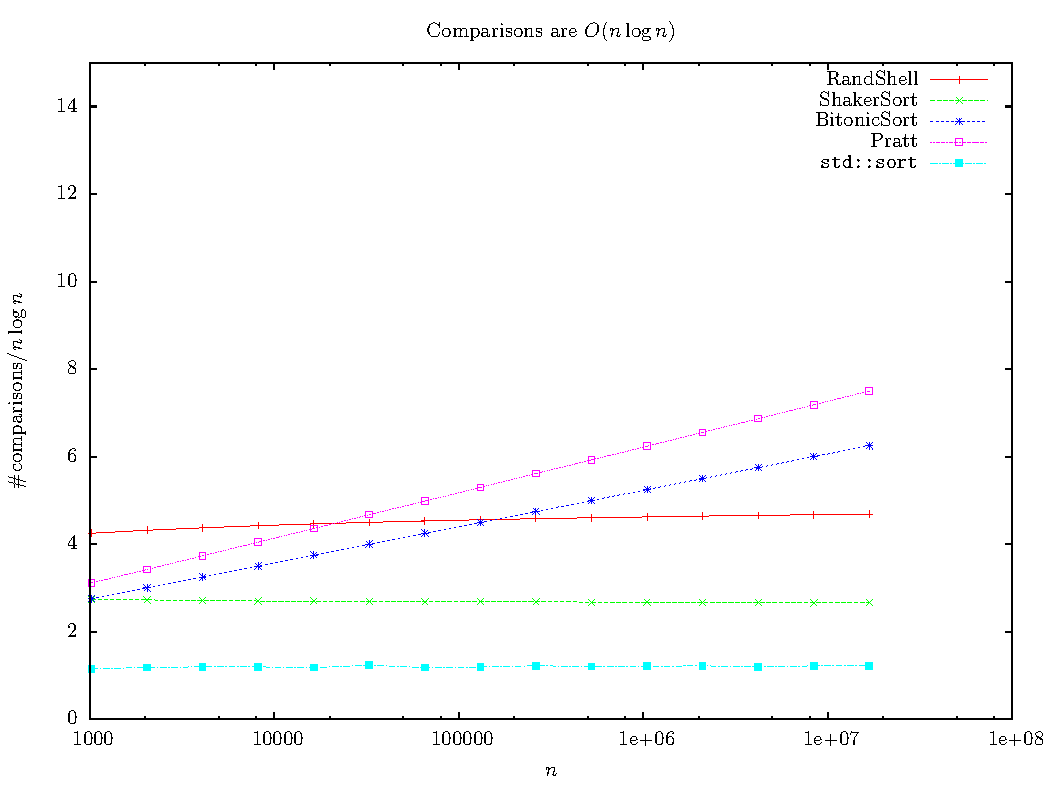
\includegraphics[width=\textwidth]{graphs/Shellsorts/nlogncomparisons.pdf}
\caption{Comparison count of the algorithms}
\label{fig:Shellsorts:comparisons}
\end{figure}

Let us then look at the running time of the algorithms, to ensure that no strange overhead is involved in sorting the data.

We see Pratt's Shellsort perform slightly worse than Bitonic Sort, but still $\Theta(n \log^2 n)$, which can be explained by a higher number of \texttt{Compare-Exchange} operations.

Shaker Sort shows great potential, performing much better than both the $\Theta(n \log^2 n)$ algorithms and Randomized Shellsort. This places Shaker Sort in a favourable position for further optimizations by applying parallel execution schemes. Keep in mind though, that the unknown failure rate for Shaker Sort might make it less desirable for practical use.
 
\begin{figure}
\center
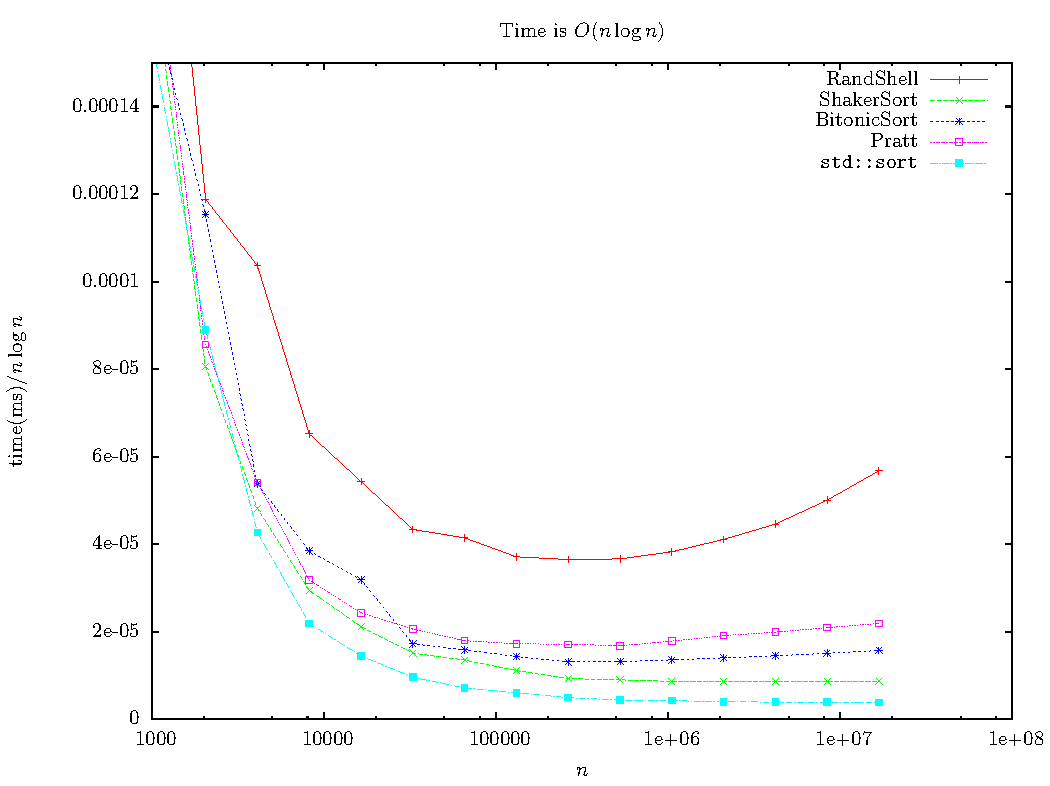
\includegraphics[width=\textwidth]{graphs/Shellsorts/nlogntime.pdf}
\caption{Running time of the algorithms}
\label{fig:Shellsorts:time}
\end{figure}

\subsection{Instructions and Cache Misses}

Now, let us look at the constant factors involved in the two Shellsort variants, and determine whether cache performance might become a problem for larger inputs, or if some of the algorithms might have an overly large instruction overhead.

Let us start by evaluating the amount of instructions per comparisons, in order to gain an insight into the performance overhead of the algorithms.

We see Pratt's Shellsort perform an amount of instructions per comparison that is slightly lower than that of Bitonic Sort, and much lower than Randomized Shellsort, while Shaker Sort is almost identical to Bitonic Sort in terms of instructions per comparison.
The low comparison overhead of the two Shellsort variants is made possible by most of their execution consisting of a few nested for-loops. 
They do however suffer from a difficulty in loop unrolling due to having their jump sequences calculated at run-time. 

\begin{figure}
\center
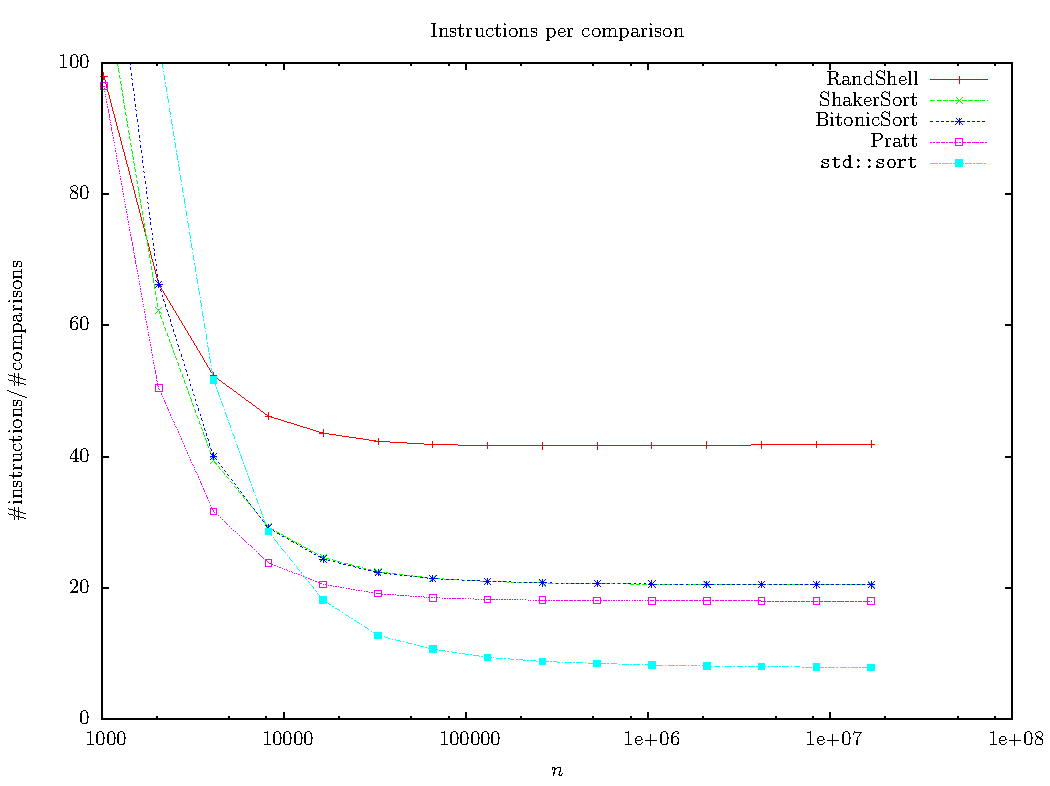
\includegraphics[width=\textwidth]{graphs/Shellsorts/instructionscomparison.pdf}
\caption{Instructions per Comparison of performed by the algorithms}
\label{fig:Shellsorts:instructions:comparisons}
\end{figure}

When looking at cache misses, we see no immediate rise in the amount of cache misses per comparison for the Shellsort variants when hitting the cache limit. This is as expected, since both of these variants of Shellsort relies entirely on performing one or two linear two-headed scans through memory per offset in the jump sequence.

\begin{figure}
\center
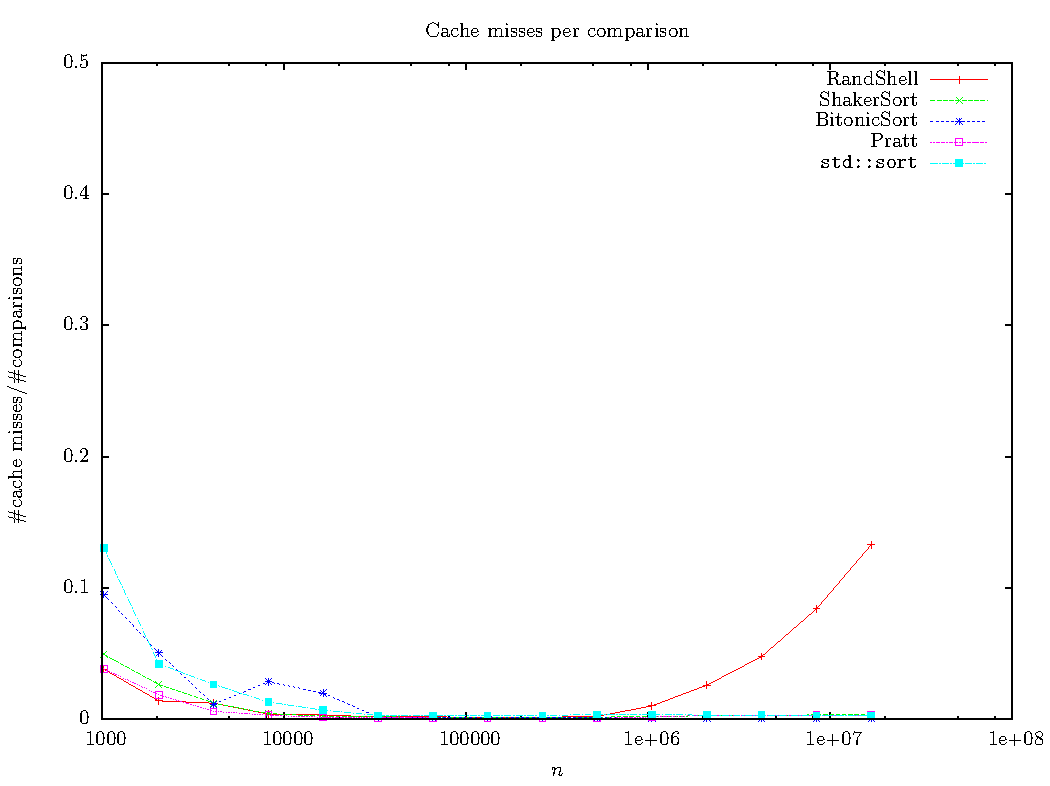
\includegraphics[width=\textwidth]{graphs/Shellsorts/cache-misses.pdf}
\caption{Cache Misses of the different algorithms}
\label{fig:Shellsorts:cachemisses}
\end{figure}

\subsection{Branch Mispredictions}

Again, let us look at the number of branch mispredictions for our data-oblivious algorithms, as they are  shown in Figure~\ref{fig:Shellsorts:branchmisses}.

We see Pratt's Shellsort and Shaker Sort perform the low amount of branch mispredictions that we have come to expect from the first experiment. Again, this is a desirable property of the algorithms when we must consider them for parallel optimization schemes.

\begin{figure}
\center
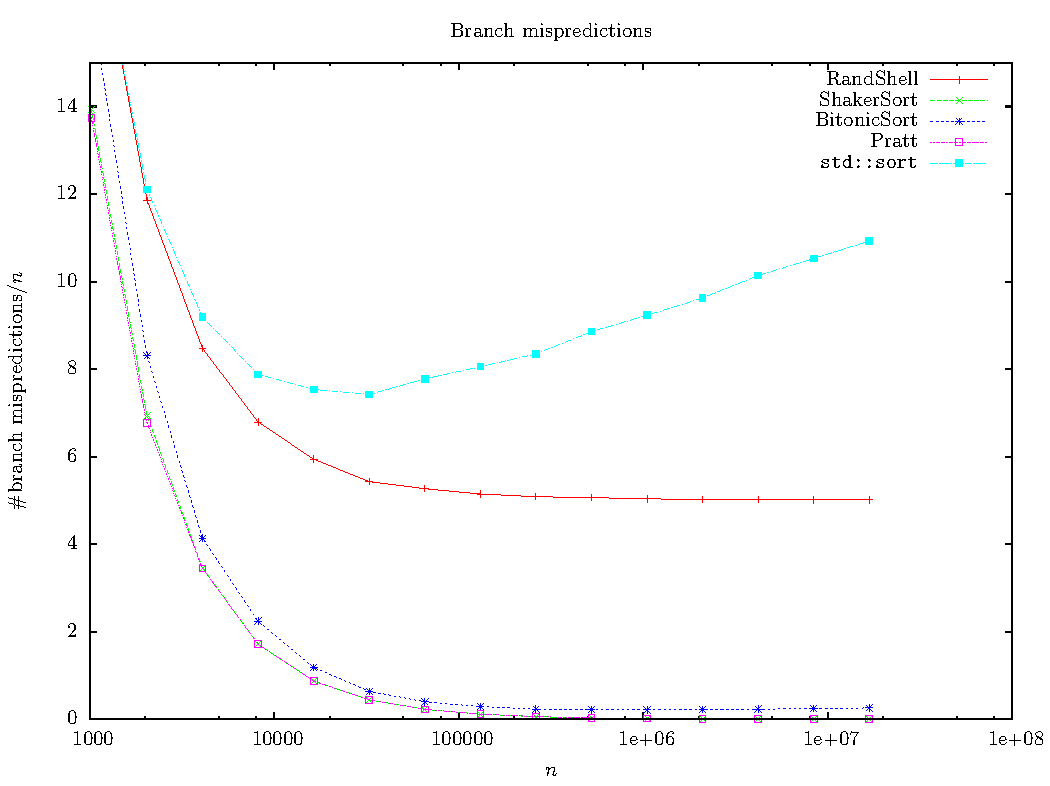
\includegraphics[width=\textwidth]{graphs/Shellsorts/branch-misses.pdf}
\caption{Branch Mispredictions of the different algorithms}
\label{fig:Shellsorts:branchmisses}
\end{figure}

\subsection{Experiment Results}

The experiment shows that both Pratt's Shellsort and Shaker Sort have excellent performance characteristics.

Pratt's Shellsort is slightly slower than Bitonic Sort, but this a by a small margin, which is a symptom of performing a slightly higher amount of comparisons.

Shaker Sort is shown to be fast in practical applications, and might be a useful data-oblivious algorithm if one ensures somewhat random input data, or accepts an unknown failure rate on certain input instances.